\section{Fresnel Zones}\label{sec:fresnel}
Taking into account that the application at hand involves radio communication it is important to talk about the Fresnel zones. The Fresnel zone is the area around the visual line-of-sight that radio waves spread out into after they leave the antenna. The radio waves will spread out into ellipse shaped areas that stretches between the two antennas. Thus, it can be seen in Figure \ref{fig:fresnel_zones} three Fresnel zones on the transmission path between A and B. 

\begin{figure}[H]
	\centering
	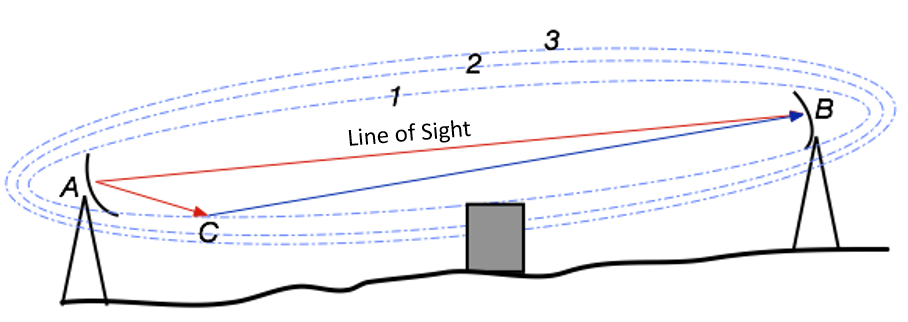
\includegraphics[scale=0.65]{figures/fresnel_zones.png}
	\caption{Fresnel zones between transmitter and receiver}
	\label{fig:fresnel_zones}
\end{figure}

On the figure above three Fresnel zones are shown, but there is an infinite number of them and the 1st zone is the one that has most effect on the performance of the Wireless Network. If there are any obstructions, such as buildings, trees or hills, located in the 1st Fresnel zone, the signal will be affected by these and would in consequence of this be weakened at the receiver.

Therefore it is a good idea when planning wireless links to keep the 1st Fresnel Zone clear of obstruction. But this can be impractical so it is said that at least 60 $\%$ (\hl{ref}) of the signal should be clear of obstructions. Although to get optimum performance it is recommended to keep the signal 20$\%$ (\hl{ref}) or less blocked. \\
%Note that obstacles in the 1st Fresnel Zone will create signals that will be 0 to 90 degrees out of phase, 90 to 270 degrees out of phase in the second zone, 270 to 450 degrees out of phase in third zone and so on.
%
%The first Fresnel zone is the ellipse with chords 1/2 wavelength longer than the direct path (ACB). 
%
%A clear line of sight is needed to maintain signal strength.%Especially for 2.4GHz wireless sytems. This is because 2.4GHz waves are absorbed by water, like the water found in trees. \hl{need something here}
%
%The direct wave, Line of Sight, goes directly from A to B and in this example it is where nothing is blocking the signal. 
%
\subsection{Fresnel zone calculations}
The following equation allows to calculate the radius of the Fresnel radius at any point P in between the endpoints of the link: 

\begin{align}
F_n = \sqrt{\frac{n \lambda d_1 d_2}{d_1+d_2}} \label{fresnel_zone_cal}
\end{align}

Where:
\begin{itemize}[label=]
\item $F_n$ = The nth Fresnel Zone radius in metres
\item d1 = The distance of P from one end in metres
\item d2 = The distance of P from the other end in metres
\item $\lambda$ = The wavelength of the transmitted signal in metres
\end{itemize}

\noindent On figure \ref{fig:fresnel_zones} the parameters from equation \ref{fresnel_zone_cal} are shown. 
\begin{figure}[H]
	\centering
	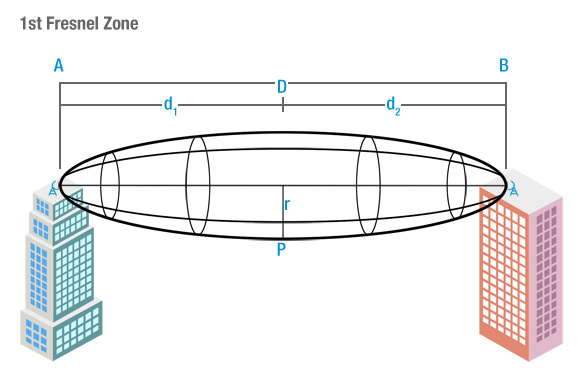
\includegraphics[scale=0.70]{figures/fresnel_zone.jpg}
	\caption{Fresnel zones}
	\label{fig:fresnel_zones}
\end{figure}  

Since the 1st Fresnel Zone is the most important, it is often useful to know the maximum radius of the zone. The radius of the Fresnel Zone is at the greatest distance at point P and therefore the distances between Point A and B to P will be identical, which implies that d1 = d2 and therefore d1 + d2 = D. Converting the wavelength value to signal frequency $\lambda = \frac{c}{f}$ the following formula for calculating the first Fresnel zone can be derived: \hl{Explain from 4.3 to 4.4}.
\begin{align}
r= 8.657 \sqrt{\frac{D}{f}} \label{eq:fresnel_radius}
\end{align}

Where:
\begin{itemize}[label=]
    \item $r$: radius in metres
    \item $D$: total distance in kilometres
    \item $f$: frequency at which are transmitted in gigahertz
\end{itemize}

\subsection{Fresnel Zones examples without curvature of the earth}
In equation \ref{eq:fresnel_radius} it is clear that by changing the distance D between the antennas, the radius r of the Fresnel zone will also change. To show how the radius changes by changing the distance, some examples are made. In these examples a frequency of 2.4Ghz are used and the curvature of the earth is not considered.

The first example shows an antenna in the height of 20 meter and a drone flying in the height of 100 meter with 10km between them.

\begin{figure}[H]
	\centering
	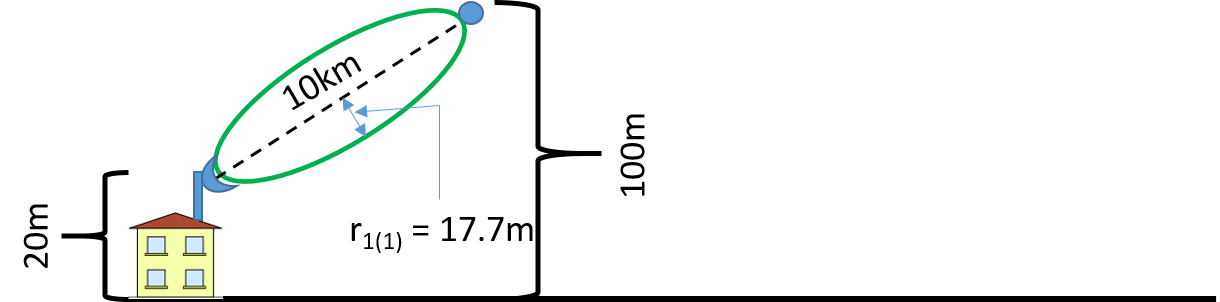
\includegraphics[scale=0.50]{figures/fresnel_10km.png}
	\caption{Fresnel zones between transmitter and receiver with a distance between them of 10km}
	\label{fig:fresnel_zones_10km}
\end{figure}  

\noindent And the radius calculated:
\begin{align*}
r1 = 8.657\cdot \sqrt{\frac{10}{2.4}} = 17.7m
\end{align*}

\noindent The second example are with a distance between them of 20km:

\begin{figure}[H]
	\centering
	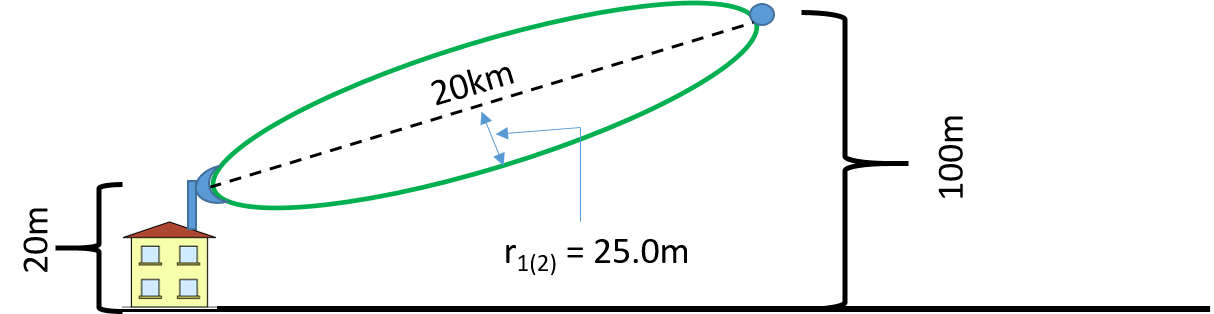
\includegraphics[scale=0.50]{figures/fresnel_20km.png}
	\caption{Fresnel zones between transmitter and receiver with a distance between them of 20km}
	\label{fig:fresnel_zones_20km}
\end{figure}  

\noindent And the radius calculated:
\begin{align*}
r2 = 8.657\cdot \sqrt{\frac{20}{2.4}} = 25.0m
\end{align*}

\noindent The third example are with a distance between them of 20km:

\begin{figure}[H]
	\centering
	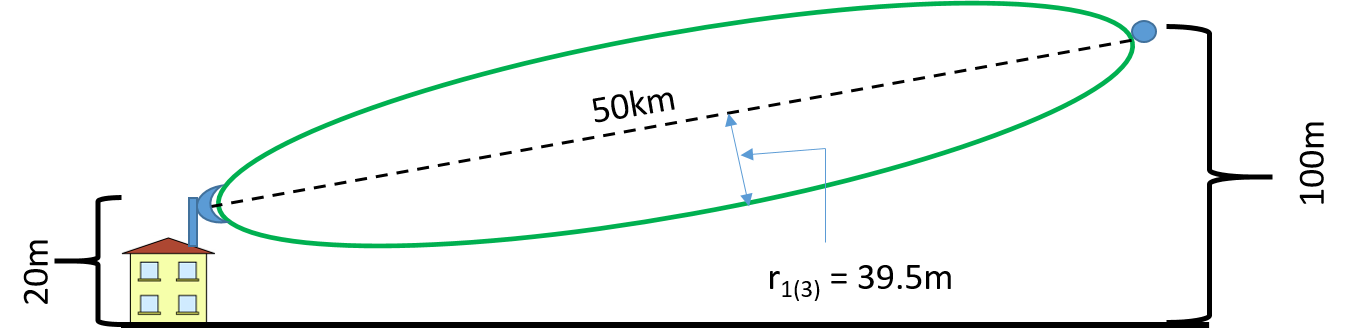
\includegraphics[scale=0.50]{figures/fresnel_50km.png}
	\caption{Fresnel zones between transmitter and receiver with a distance between them of 50km}
	\label{fig:fresnel_zones_50km}
\end{figure}  

\noindent And the radius calculated:
\begin{align*}
r3 = 8.657\cdot \sqrt{\frac{50}{2.4}} = 39.5m
\end{align*}

\noindent In these examples it is demonstrated that the radius of the Fresnel Zone increases when the distance between the antennas increases.

\subsection{60\% Clearance Zone of the 1st Fresnel Zone}
\hl{Lets} try to find out how tall a structure could be at the center of the Fresnel Zone, if 60\% should be clear of this zone, i.e 40\% should be blocked. For this the following equation must be used:

\begin{align*}
r = 8.657\cdot \sqrt{\frac{0.6D}{f}}
\end{align*}

\hl{Lets} assume that both antennas are at a height of 20 meters and operating at 2.6GHz:

\begin{align*}
\text{radius} = 8.657\cdot \sqrt{\frac{10}{2.4}} = 17.7m
\end{align*}

Here the first Fresnel zone would pass just 2.3 meters above ground level in the middle of the link. 

\begin{figure}[H]
	\centering
	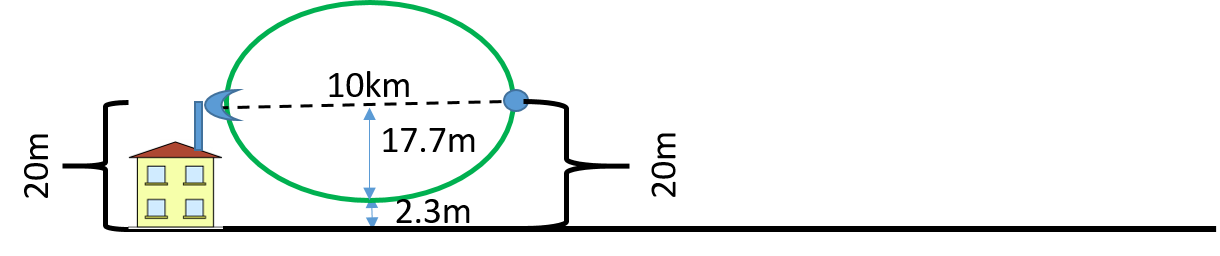
\includegraphics[scale=0.50]{figures/fresnel_10km_height.png}
	\caption{Fresnel zones between transmitter and receiver  with a distance between them of 10km. The antennas have same height above ground level.}
	\label{fig:fresnel_zones_10km_height}
\end{figure}  

\noindent Now \hl{lets} calculate how tall a structure should be if 60\% of the signal should be cleared:

\begin{align*}
\text{radius} = 8.657\cdot \sqrt{0.6\cdot \frac{10}{2.4}} = 13.7m
\end{align*}
  
\noindent By subtracting this result from the antenna height, the maximum height of any obstruction between the devices within 60\% clear Fresnel Zone can be calculated:

\begin{align*}
\text{Maximum Obstruction Height} = 20 - 13.7 = 6.3m
\end{align*}

Therefore the maximum permissible height of any obstruction located between the two antennas, 10km apart, operating at 2.4GHz, at antenna heights of 20m with a minimum clearance Fresnel Zone of 60\% is 6.3m. An illustration of this is shown in figure \ref{fig:fresnel_zones_10km_60procent}.

\begin{figure}[H]
	\centering
	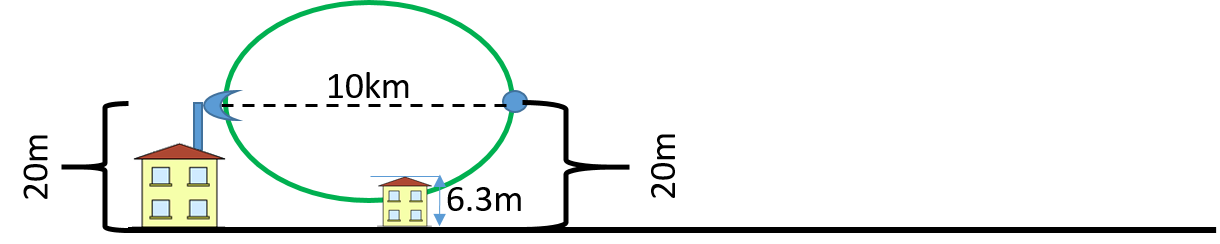
\includegraphics[scale=0.50]{figures/fresnel_10km_60procent.png}
	\caption{Fresnel zone between transmitter and receiver in 10km distance. With a obstacle where 40\% of the signal is blocked.}
	\label{fig:fresnel_zones_10km_60procent}
\end{figure}  

\noindent An obstruction higher than 6.3m will give less than 60\% clearance of the Fresnel Zone. To prevent this problem, the antenna need to be positioned higher up, the frequency could be changed or the direction of the link should be changed to avoid obstacles.

\subsection{Fresnel zones examples with curvature of the earth}
For longer distance links the curvature of the earth comes into play and may become an obstruction into the Fresnel zone and cause signal loss. This is because that the longer the distance between the antennas the greater the radius of the Fresnel zones. The formula for calculating the effect of the Earth's radius is as follows(\hl{ref}):

\begin{align}
H = \frac{1000\cdot D^2}{8\cdot E_r}
\end{align}

Where:
\begin{itemize}[label=]
    \item $H$: Height difference of Earth's Curvature at the mid-point between the two devices (m)
    \item $D$: Total Link Distance between the two devices (km)
    \item $E_r$:  Effective Radius of Earth (km) Note: Usually taken as 4/3 (1.333 rec.)actual radius to account for atmospheric refraction i.e. 8,504km
\end{itemize}

\noindent The best way to show how this comes into play is by showing an example. An illustration about the Fresnel zones, where the curvature of the earth is taking into account is shown on figure \ref{fig:fresnel_50km_curvature}. On this figure the building and the drone is at 77m height and is at a distance of 50km from each others. 

\begin{figure}[H]
	\centering
	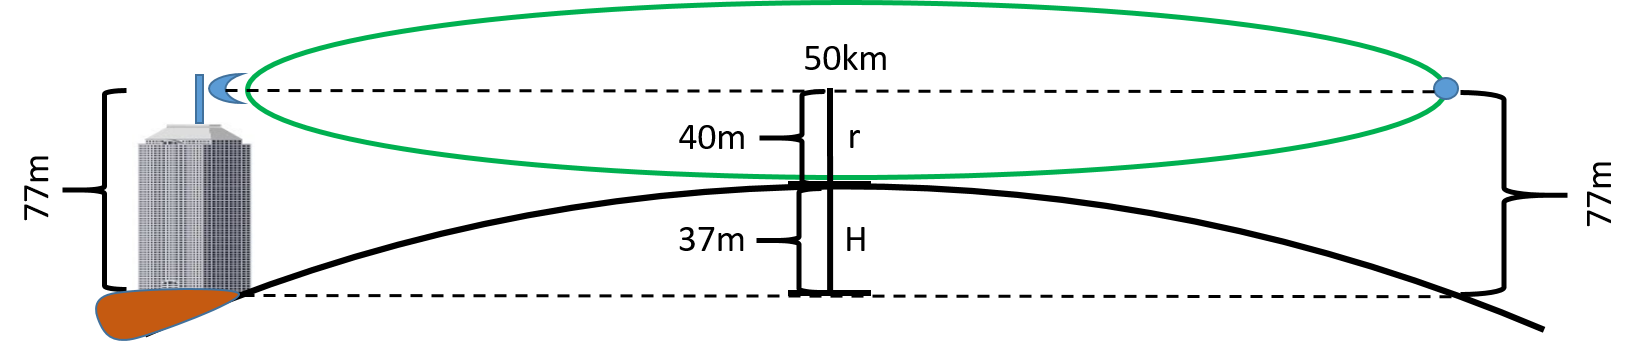
\includegraphics[scale=0.50]{figures/fresnel_50km_curvature.png}
	\caption{Fresnel zone in 50km distance. With curvature of the earth taken into account.}
	\label{fig:fresnel_50km_curvature}
\end{figure}  

\noindent The height difference of the earth's curvature at the mid-point between the drone and the building:
\begin{align}
\text{H} = \frac{1000 D^2}{8 \cdot E_r} = \frac{1000 \cdot 50^2}{8\cdot 8504} = 36.7m \approx 37m
\end{align}

\noindent The radius of the 1st Fresnel zone:
\begin{align*}
\text{r} = 8.657\cdot \frac{0.6\cdot D}{f} = 8.657\cdot \frac{50}{2.4} = 39.5m \approx 40m 
\end{align*}

\noindent Maximum height of the obstruction between the two devices within the 60\% clearance zone:

\begin{align*}
\text{radius}_{60} &= 8.657\cdot \frac{D}{f} = 8.657\cdot \frac{0.6\cdot 50}{2.4} = 30.6m \approx 31m \\
\text{Obs}_{\text{max height}} &= 77m - \text{radius}_{60} = 77m - 31m = 46m \\
\text{height}_{\text{max with curv}} &= \text{Obs}_{\text{max height}} - H = 46m - 37m = 9m
\end{align*}

\noindent On figure \ref{fig:fresnel_50km_curvature_obstacle} an obstruction is added with the above calculations added:

\begin{figure}[H]
	\centering
	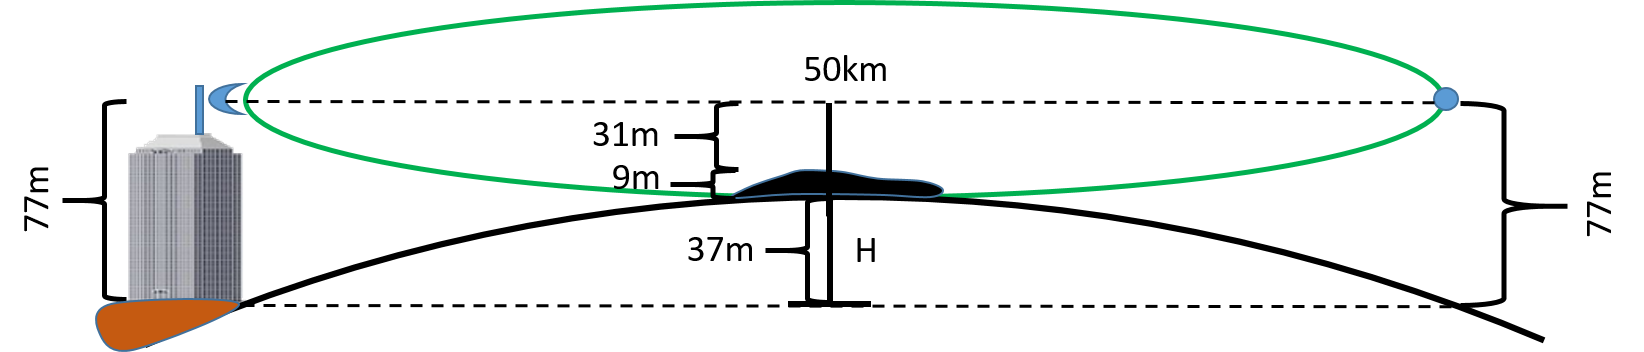
\includegraphics[scale=0.50]{figures/fresnel_50km_curvature_obstacle.png}
	\caption{Fresnel zone in 50km distance. To have 60\% clearance of the Fresnel zone. With curvature of the earth taken into account.}
	\label{fig:fresnel_50km_curvature_obstacle}
\end{figure}  

